\documentclass[12pt]{article}
\usepackage{mathtools}
\usepackage{fontspec}
% \usepackage[left=1.06cm,top=0.9cm,right=1.06cm,bottom=0.49cm]{geometry}
% \setmainfont{GFS Didot}
\setmainfont{EB Garamond}


% Set page size and margins
% Replace `letterpaper' with `a4paper' for UK/EU standard size
\usepackage[a4paper,top=2cm,bottom=1.5cm,left=1cm,right=1cm]{geometry}
\usepackage{fancyhdr}
\pagestyle{fancy}
\setlength{\parindent}{0pt}


% Useful packages
\usepackage{graphicx}
\graphicspath{{./media/}}
\usepackage{subfig}
\usepackage{float}
\usepackage[colorlinks=true, allcolors=blue]{hyperref}
\usepackage{siunitx}
\usepackage{sectsty}
\sectionfont{\fontsize{12}{15}\selectfont}

\title{\vspace{-2cm}033 - Διατάξεις Υψηλών Συχνοτήτων \\ 
        \large 1η Σειρά Ασκήσεων}
\author{Ιωάννης Δημουλιός \\ 
        \large 10641}
\date{Εαρινό εξάμηνο 2024}

\lhead{033-Διατάξεις Υψηλών Συχνοτήτων}
\chead{1η Σειρά Ασκήσεων}
\rhead{Ιωάννης Δημουλιός}
\begin{document}
\maketitle
\section*{1.1. Ανάλυση κυκλώματος γραμμής μεταφοράς - Διάγραμμα Smith}
\textbf{(α)} Κανονικοποιώντας ως προς \(Z_0 = \SI{50}{\ohm}\), παίρνουμε \(z_L = 2\) και 
\[
z_{cap} = \dfrac{-j}{2\pi f_0 C Z_0} = -j1.592
\]
Από το διάγραμμα Smith προκύπτει: 
\begin{gather*}
    \Gamma = \dfrac{\SI{3.35}{\cm}}{\SI{8}{cm}} = 0.4185 \\
    SWR = 2.44
\end{gather*}
\begin{center}
    \includegraphics*[scale=0.5]{1-1-a.jpg}
\end{center}

\newpage
\textbf{(β)} Με όμοιο τρόπο \(z_L = 2\), \(z_{cap} = -j1.194\). Τα μήκη των γραμμών ως προς το νέο μήκος κύματος γίνονται: 
\begin{gather*}
    0.32\lambda_0 \rightarrow 0.427\lambda \\
    0.24\lambda_0 \rightarrow 0.32\lambda \\ 
    0.1\lambda_0 \rightarrow 0.133\lambda
\end{gather*}
Πάλι από το διάγραμμα Smith: 
\begin{gather*}
    \Gamma = \dfrac{2.75}{8} = 0.34375 \\ 
    SWR = 2.05
\end{gather*}
\begin{center}
    \includegraphics*[scale=0.5]{1-1-b.jpg}
\end{center}

\textbf{(γ)} Αν γραμμή ήταν ΤΕΜ ή quasi-TEM, θα έπρεπε να δοθεί η σχέση διασποράς \(\beta(f)\), για να υπολογιστούν τα νέα ηλεκτρικά μήκη των γραμμών μεταφοράς. 

\newpage
\section*{1.2. Ανάλυση κυκλωμάτων γραμμών μεταφοράς στο πεδίο της συχνότητας}

\textbf{(α)}

\begin{center}
    \includegraphics*[scale=0.65]{1-2-a.png}
\end{center}
Η προσομοίωση επιστρέφει για 
\begin{itemize}
    \item \(f_0 = \SI{1}{GHz} \qquad \Gamma = 0.413 \quad SWR = 2.406\)
    \item \(f_1 = \SI{1.33}{GHz} \qquad \Gamma = 0.371 \quad SWR = 2.179\)
\end{itemize}
Και οι τέσσερις τιμές βρίσκονται ικανοποιητικά κοντά σε αυτές που υπολογίσαμε με τα διαγράμματα Smith. 
\bigskip

\textbf{(β)}
\begin{center}
    \includegraphics*[scale=0.65]{1-2-b_0.png}
\end{center}

Δεδομένου ότι οι αποδεκτές τιμές του συντελεστή ανάκλασης και του λόγου στάσιμου κύματος είναι αντίστοιχα \[\Gamma_{dB} \leq \SI{-10}{dB},\quad SWR \leq 3\]
τo φίλτρο χαρακτηρίζεται ως χαμηλοπερατό. 

\newpage
Πέραν της άσκησης βέβαια, αν μεγαλώσουμε το εύρος συχνοτήτων της ανάλυσης λαμβάνουμε: 
\begin{center}
    \includegraphics*[scale=0.5]{1-2-b_1.png}
\end{center}
Όπως φαίνεται από τα γραφήματα, η απόκριση του φίλτρου είναι περιοδική με περίοδο \(\SI{4}{GHz}\).
\bigskip

\textbf{(γ)} 
\begin{center}
    \includegraphics*[scale=0.65]{1-2-c.png}
\end{center}
Και αυτό το φίλτρο χαρακτηρίζεται ως χαμηλοπερατό. 

\newpage
\section*{1.3. Συζυγής προσαρμογή – Διάγραμμα Smith}
\textbf{(α)}
\begin{center}
    \includegraphics*[scale=0.7]{1-3-a.jpg}
\end{center}

To διάγραμμα Smith καλύπτει όλες τις περιπτώσεις.
Για να πετύχουμε συζυγή προσαρμογή, θέλουμε 
\[
    z_{in} = z^*_g = 1 + j0.8
    \]
Οπότε προκύπτει ότι για: 

\begin{itemize}
    \item \textit{Πυκνωτή σε σειρά με το φορτίο} δεν υφίσταται λύση, εφόσον ο κύκλος σταθερού $r = 0.2$, πάνω στον οποίο κινούμαστε λόγω του πυκνωτή ξεκινώντας από $z_L$, δεν τέμνει τον κύκλο σταθερού $SWR = 2.2$, πάνω στον οποίο θα κινούμασταν λόγω την γραμμής μεταφοράς, για να καταλήξουμε στο $z^*_g$.
    \item \textit{Πυκνωτή παράλληλο στο φορτίο} η χωρητικότητα του πυκνωτή και το μήκος της γραμμής πρέπει να είναι αντίστοιχα
        \begin{gather*}
            b = - 0.84 - (-2.31) = 1.47 \implies C = \dfrac{b}{2\pi f_0 Z_0} = \SI{4.7}{pF} \\
            \ell = 0.406\lambda - 0.307\lambda = 0.099\lambda
        \end{gather*}
    \item \textit{Πυκνωτή παράλληλο στην είσοδο} 
        \begin{gather*}
            b = - 0.49 - (-1.43) = 0.94 \implies C = \dfrac{b}{2\pi f_0 Z_0} = \SI{3.0}{pF} \\
            \ell = 0.337\lambda - 0.298\lambda = 0.039\lambda
        \end{gather*}
    \item \textit{Πυκνωτή σε σειρά με την είσοδο}
        \begin{gather*}
            x = 1.93 - 0.8 = 1.13 \implies C = \dfrac{1}{2\pi f_0 Z_0 x} = \SI{2.8}{pF} \\
            \ell = 0.186\lambda - 0.048\lambda = 0.138\lambda
        \end{gather*}
\end{itemize}
\textbf{(β)} H ισχύς στο φορτίο είναι ίση με την ισχύ εισόδου και υπολογίζεται ως εξής: 
\[
    P = \dfrac{V^2_{s, \text{rms}}}{4R_g} = \dfrac{1}{4\cdot 50} = \SI{5}{mW}
\]

\textbf{(γ)} 
\begin{center}
    \includegraphics*[scale=0.5]{1-3-c_A.png}
    \includegraphics*[scale=0.5]{1-3-c_B.png}
    \includegraphics*[scale=0.5]{1-3-c_C.png}
\end{center} 
Και αθροιστικά 
\begin{center}
    \includegraphics*[scale=0.6]{1-3-c_all.png}
\end{center} 

Η ευθεία στα \(\SI{2.5}{mW}\) υποδεικνύει τη μισή ισχύ της μέγιστης σε όλα τα γραφήματα.

Εμφανώς, το μεγαλύτερο εύρος ζώνης προκύπτει στην περίπτωση που έχουμε τον \textbf{\textit{Πυκνωτή παράλληλα στο φορτίο}}.

\newpage
\section*{1.4. Πολλαπλός κλαδωτής}
\textbf{(α)} Δείτε τις συναρτήσεις 
\begin{itemize}
    \item \texttt{reflectionCoefMultiStub(freqRatio, p)},
    \item \texttt{reflectionCoefMultiStubSimulation(p)},
    \item \texttt{reflectionCoefMultiStubSimulationMean(p)}
\end{itemize}
στο συνημμένο αρχείο \texttt{src/multiStub.jl}. 

\bigskip
\textbf{(β)} Δείτε το αρχείο \texttt{src/optimMultiStub.jl}.

\bigskip
\textbf{(γ)} 
Δείτε τη συνάρτηση \texttt{reflectionCoefMultiStubSimulationPlot(p)} στο \texttt{src/multiStub.jl}.  \\
Από τα διάφορα διανύσματα \(p\) που επέστρεψε ο γενετικός αλγόριθμος η ελάχιστη μέση τιμή του συντελεστή ανάκλασης προέκυψε για  
\[
    p_{\text{optimal}} = 
    \begin{bmatrix}
         0.2501613826522009 \\
 0.052410648861077894 \\
 0.09937524072518232  \\
 0.4643724374109345 \\
 0.07818274587913998 \\
 0.04842408964473821
    \end{bmatrix}
\] 
και ήταν η 
\[
    |\Gamma|_\text{mean} = 0.387216493658603
\]
Στο εύρος συχνοτήτων \(0.01f_0\) με \(2f_0\) για το \(p_{\text{optimal}}\)
η γραφική παράσταση του συντελεστή ανάκλασης γίνεται: 
\begin{center}
    \includegraphics*[scale=0.6]{1-4-c.png}
\end{center}

\textbf{(δ)} 
Το βέλτιστο \(|\Gamma|_\text{mean} = 0.48949835544438386\) προκύπτει για: 
\[
    p_{\text{optimal}} = 
    \begin{bmatrix}
         0.23543805815455376 \\
 0.17665521925177036 \\
 0.19008167398643355 \\
 0.0643011430492405 \\
 0.042261233507735585 \\
 0.03111688618348929
    \end{bmatrix}
\] 
Ωστόσο, από τη γραφική παράσταση φαίνεται ότι το εύρος συχνοτήτων για το οποίο \(|\Gamma| \leq 0.3\) είναι πολύ μικρό, γεγονός το οποίο φυσικά είναι ανεπιθύμητο. 
\begin{center}
    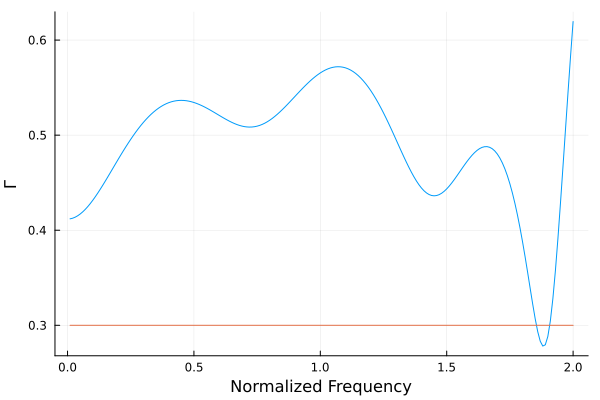
\includegraphics[scale=0.5]{1-4-d.png}
\end{center}

\textbf{(ε)} Για \(Z_L = 20 + j30\) ο γενετικός αλγόριθμος δίνει \(|\Gamma|_\text{mean} = 0.4175269577424611\) για 
\[
    p_{\text{optimal}} = 
    \begin{bmatrix}
        0.0 \\
        0.17104122220366383 \\
        0.17423539738754057 \\
        0.08019708285438065 \\
        0.050788540175335184 \\
        0.03552256267842435 \\
    \end{bmatrix}
\] 
Παρ' όλο που μειώθηκε αισθητά ο μέσος όρος τώρα δεν υπάρχει εύρος συχνοτήτων για το οποίο \(|\Gamma| \leq 0.3\). 
Επίσης παρατηρούμε ότι τώρα το \(d_1 = 0.0\), δηλαδή για να επιτευχθεί ο βέλτιστος συντελεστής ανάκλασης πρέπει το φορτίο να μην απέχει από την αρχή του πρώτου κλαδωτή. 

\begin{center}
    \includegraphics*[scale=0.5]{1-4-e_A.png}    
\end{center}

\newpage
Για \(Z_L = 180 - j200\) λαμβάνουμε \(|\Gamma|_\text{mean} = 0.7233702757921985\) για 
\[
    p_{\text{optimal}} = 
    \begin{bmatrix}
        0.16592399862317087 \\
        0.05 \\
        0.050623765157369674 \\
        0.35704408661476317 \\
        0.0719505995319416 \\
        0.02816161313633092 \\
    \end{bmatrix}
\]

Και πάλι ο συντελεστής ανάκλασης βρίσκεται σε αποδεκτές τιμές για πολύ μικρό εύρος συχνοτήτων. 

\begin{center}
    \includegraphics*[scale=0.5]{1-4-e_B.png}
\end{center}

\underline{\textbf{Σημείωση}} \\
Αν στόχος μας, αντί για την ελαχιστοποίηση της μέσης τιμής του συντελεστή ανάκλασης, ήταν η μεγιστοποίηση του εύρους συχνοτήτων με αποδεκτό συντελεστή ανάκλασης, θα μπορούσαμε να χρησιμοποιήσουμε διαφορετικά μέτρα προσαρμογής. Ενδεικτικά, δείτε τις συναρτήσεις στο \texttt{src/multiStub.jl} 
\begin{itemize}
    \item \texttt{bandwidthCounter(p)} για τη μεγιστοποίηση των σημείων στο φάσμα συχνοτήτων της προσομοίωσης που παράγουν αποδεκτό συντελεστή ανάκλασης
    \item \texttt{bandwidthCounterWeighted(p)} που εξυπηρετεί το ίδιο με την προηγούμενη, αλλά ενθαρρύνει τα σημεία να είναι διαδοχικά. 
\end{itemize} 
Παρατίθενται και τα σχετικά γραφήματα για το αρχικό φορτίο \(Z_L = 120 + j60\). 

\begin{figure}[H]
    \centering
    \subfloat{{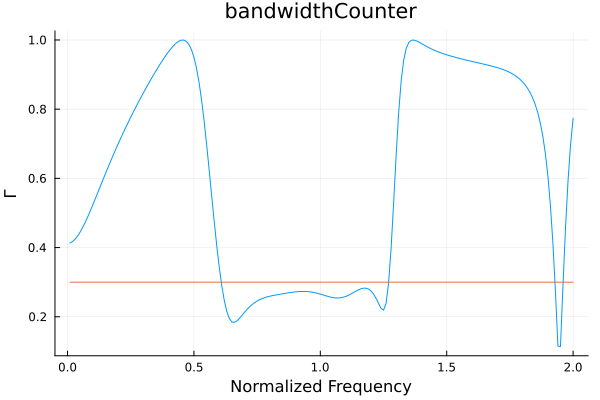
\includegraphics[scale=0.42]{1-4-bonus_A.png} }}
    \qquad
    \subfloat{{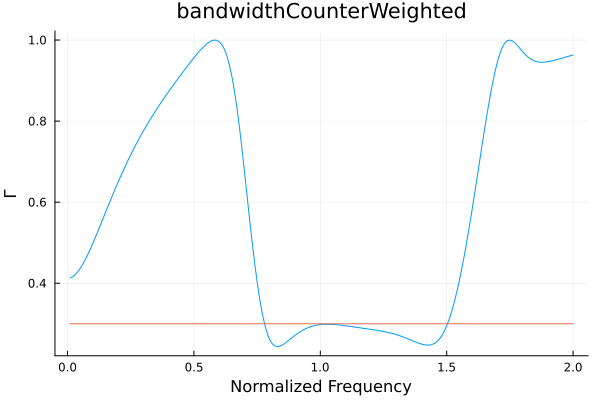
\includegraphics[scale=0.42]{1-4-bonus_B.png} }}
\end{figure}

\end{document}
